\section{Introduction}
\label{sec:intro}

Task-specific  conversational  chatbot  \cite{wen2016network}  has been applied into  many practical products. 
A popular one is the smart speaker, e.g. Alex, Siri, Google home. 
Another important one is the customer service system, which greatly help human agents handle miscellanious customer's questions.
No matter these applications involves single- or  multi-round conversations, a critical step is to identify  the  intent  behind  a  user's  question or response. 
The detected intent  with  its  associated  attributes is then mapped into a predefined dialog logic to obtain a suitable response to return to customers.

In  the early stage  of  building  a  chatbot , sufficient  labeled  data is often expensive to obtain to render the system to achieve a strong performance.
People thus have to filter out enough typical users' utterances from tons of real conversation logs, and label them  with proper intents. 
In practice, this procedure can be improved by active-learning like operations. 
A basic intent detection system with very limited manually labeled data can be built first, and then it filters out a set of potential data with high confidences for humans to label.
The new data is added to train a better system again. 
This procedure iterates until the system reach a high performance.
Therefore, it is meaningful to address the challenge of short-text classification   \cite{sriram2010short, chen2019deep, phan2008learning,yan2009dynamic,hua2015short}   problem   under the few-shot   setting \cite{yu2018diverse}.

Existent approaches for intent detection can be roughly categorized as text classfication model and text similarity model.

The first one,  \emph{text  classification model},  includes a variety of work.
From  traditional  machine  learning models like SVM \cite{suykens1999least}, boosting tree  \cite{tu2005probabilistic},  to neural networks \cite{wen2016network}, such as   convolutional      neural     networks (CNNs) \cite{kim2014convolutional,zhang2015character,conneau2016very}  and  long  short term  memory  networks  (LSTMs)  \cite{mousa2017contextual,liu2016recurrent}, and then to the most popular pretrained language models based, such as BERT \cite{devlin2018bert}, RoBERTa  \cite{liu2019roberta} and etc. 
Especiallaly, pretrained     models     based    \cite{vaswani2017attention}  tends to be more helpful in the few-shot scenario \cite{yu2018diverse, madabushi2020cost}  to alleviate the dearth of training data.
Another two interesting lines of work, label-word joint models, and joint NER and classification are discussed in the related work of appendix.

The  second  one, \emph{text similarity model}, is usually employed to calculate how  similar  between an input text and a historical text in the repository. 
The associated label of the most similar historical text is returned as the label of the  text  to  query \cite{jafarpour2010filter,   leuski2011npceditor}.  
A  popular  and  effective  methodology  is adopting pretrained models to model the similarity calculation as a binary classification problem.

Despite  plenty of success  of  these two methodologies, they still have some limitations in this task especially when data is insufficient.
Regarding  the  \emph{text  classification  model}, it learns a function that directly maps an input query into its expected label.
Its training requires data in the form of a pair of  a query and a task dependent label. 
It is quite hard to adopt labeled data from other domains, as their label definitions are often incompatible to each other. 
Though we can use some data augmentation methods to alleivate the paucity of data,  e.g., translation based paraphrasing methods, the resulting benefit is still limited because of the data being homogeneous, in the case that our labeled data is very insufficient.
Regarding the  \emph{similarity model}, the foremost advantage is it does not pose any restriction on the label definition of user intents, but aims to learn a function that measure how similar of two sentences are. 
Then in the intent detection task, we are only concerned which labeled query is the most similary one to the current input, and then use its label as the output.
This results in a possibility that even though the labeled data in current domain is scarce, we may borrow additional data from another domain to help enhance the similarity model to make a better intent prediction.
Nevertheless, just as every coin has two sides, the high flexibility of similarity model leads to its worse performance compared to a classification model,  because its training loss differs from a classification loss corresponding to the intent detection goal.
More, it requires an auxiliary model to narrow down candidate labeled queries to speed up the calculation, which makes it slow in the speed and tricky in the auxiliary model selection. 

The  above  limitations motivate us to propose a system that may take both the high performance from a classification model and the ability of supporting out-of-domain data from a similarity model.
We call our system as SFC,  short  for  similarity model fused with classification model, shown in Fig.  \ref{fig:framework}.  
In order to train effectively, we further borrow the multi-task learning   \cite{caruana1993multitask,collobert2008unified,  liu2019multi}.
Our basic  idea  come naturally, and the first impementation consists of two stages. 
In the first stage, we use an auxiliary model to  select  top-K most possible labels for an input. 
This model can be an elastic search  \cite{divya2013elasticsearch}  or a text classification model trained on current domain.  
In  the  second  stage,  we  build  a classification  model  which is composed of several similarity  modules. 
Then, this structure  derives  two  goals to train towards, the task-specific classification loss ,  and  the similarity loss on both in-domain and out-of-domain data. 
In this version, the two stages are  independently optimized, so we call it \emph{two-stage SFC}. 

We further find that the  quality of outputs from the first stage might limit the final performance of the system,  since  those outputs are fixed in the whole system training  procedure.  
This  observation motivates us to continue improving  the  above two-stage  SFC  into a joint training setting, and we call this second version as \emph{joint SFC}. 
In this  way, the first stage model can be optimized by the optimization in the second stage so that it can provide better candidates to improve the performance of the second stage in turn.

Experiment  results  from  6  public  and  1  private  short-text classification datasets,  show  that  our proposed SFC joint system can achieve significant and consistent  improvements  over  strong baselines, especially in the low resource settings.

\begin{figure*}[t]
  \begin{centering}
    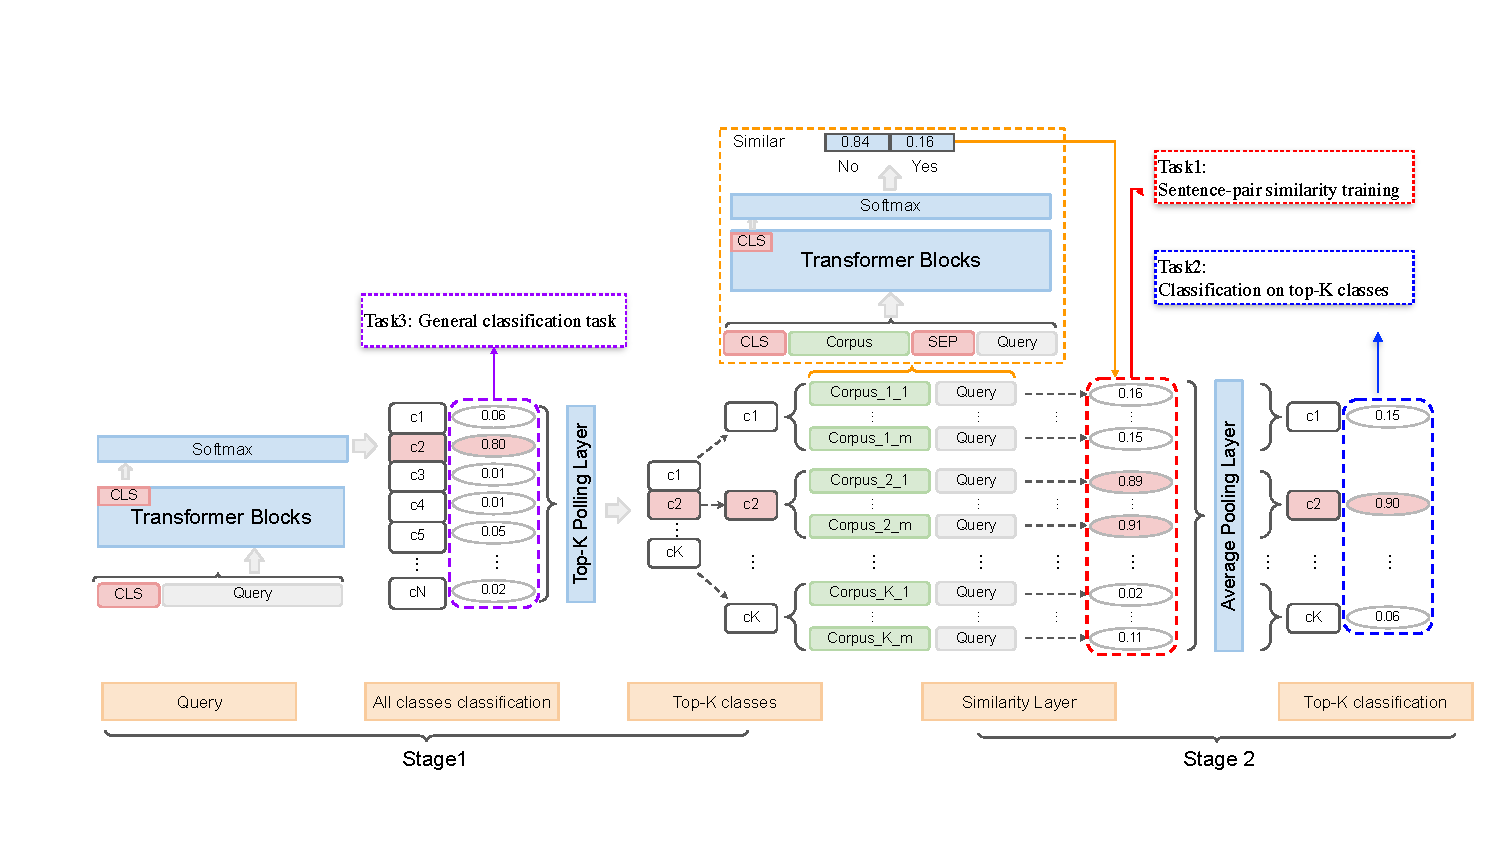
\includegraphics[scale=0.66]{picture/picture4} 
    \par
  \end{centering}
  \caption{
    \textbf{Network Structure of SFC:} two-stage SFC and joint-SFC are sharing
    the  same  network  from  stage  1  and  stage 2, with the only difference
    whether two stages being jointly trained.
  }
  \label{fig:framework}
\end{figure*}

